\documentclass{beamer}
\usepackage{booktabs, calc, rotating, url}
% This file is a solution template for:

% - Giving a talk on some subject.
% - The talk is between 15min and 45min long.
% - Style is ornate.



% Copyright 2004 by Till Tantau <tantau@users.sourceforge.net>.
%
% In principle, this file can be redistributed and/or modified under
% the terms of the GNU Public License, version 2.
%
% However, this file is supposed to be a template to be modified
% for your own needs. For this reason, if you use this file as a
% template and not specifically distribute it as part of a another
% package/program, I grant the extra permission to freely copy and
% modify this file as you see fit and even to delete this copyright
% notice.

\DeclareMathOperator{\dif}{d \!}
\newcommand{\bm}[1]{{\boldsymbol {#1}}}
\newcommand{\bZ}{{\bm Z}}
\newcommand{\bz}{{\bm z}}
\newcommand{\bY}{{\bm Y}}
\newcommand{\by}{{\bm y}}
\newcommand{\bX}{{\bm X}}
\newcommand{\bx}{{\bm x}}
\newcommand{\bh}{{\bm h}}

\newcommand{\bmu}{{\mathbf \mu}}
\newcommand{\bdelta}{{\mathbf \delta}}
\newcommand{\bepsilon}{{\mathbf \epsilon}}

\newcommand{\Cov}{\mathrm{Cov}}%
\newcommand{\transp}{\top}
\newcommand{\diag}{\,\mathrm{diag}\,}%

\newcommand{\truez}{true}
\newcommand{\bfalpha}{\mbox{\boldmath{$\alpha$}}}
\newcommand{\bfbeta}{\mbox{\boldmath{$\beta$}}}
\newcommand{\bftheta}{\mbox{\boldmath{$\theta$}}}


\mode<presentation>
{
  %\usetheme{AnnArbor}
  \usetheme{IowaCity}
  % or ...

  \setbeamercovered{transparent}
  % or whatever (possibly just delete it)
}


\usepackage[english]{babel}
% or whatever

\usepackage[latin1]{inputenc}
% or whatever

\usepackage{times}
\usepackage[T1]{fontenc}
% Or whatever. Note that the encoding and the font should match. If T1
% does not look nice, try deleting the line with the fontenc.


\title % (optional, use only with long paper titles)
{Penalized Regression with Various Design Matrix Correlation Structures}

% \subtitle
% {Presentation Subtitle} % (optional)

\author{Hao Chai\inst{}}
% - Use the \inst{?} command only if the authors have different
%   affiliation.

\institute[U of Iowa] % (optional, but mostly needed)
{
  \inst{}
   Department of Statistics and Actuarial Science \\
  The University of Iowa
}
% - Use the \inst command only if there are several affiliations.
% - Keep it simple, no one is interested in your street address.

\date[] % (optional)
{\today}

\subject{Talks}
% This is only inserted into the PDF information catalog. Can be left
% out.



% If you have a file called "university-logo-filename.xxx", where xxx
% is a graphic format that can be processed by latex or pdflatex,
% resp., then you can add a logo as follows:

\pgfdeclareimage[height=0.5cm]{university-logo}{ui-dome.jpg}
\logo{\pgfuseimage{university-logo}}



% Delete this, if you do not want the table of contents to pop up at
% the beginning of each subsection:
% \AtBeginSubsection[]
% {
%   \begin{frame}<beamer>
%     \frametitle{Outline}
%     \tableofcontents[currentsection,currentsubsection]
%   \end{frame}
% }

\AtBeginSection[]
{
  \begin{frame}<beamer>
    \frametitle{Outline}
    \tableofcontents[currentsection]
  \end{frame}
}

% If you wish to uncover everything in a step-wise fashion, uncomment
% the following command:

%\beamerdefaultoverlayspecification{<+->}



\begin{document}

\begin{frame}
  \titlepage
\end{frame}

\begin{frame}
  \frametitle{Outline}
  \tableofcontents
  % You might wish to add the option
  [pausesections]
\end{frame}


\section{Comparison among Three Covariance Structures}
\begin{frame}
\frametitle{Problem Review}
The goal is to minimize $$||\mathbf{y}-X\bm\beta||^2_2+\sum_{i=1}^p\rho(|\beta_i|;\lambda).$$
\pause
Want to compare the performance of LASSO and MCP under different correlation structures.

Set $\bm\beta=(3, 1, -1, 3, \mathbf{0})$, $n=100$, $p=500$ and signal to noise ratio $s/n = 1.5$.

There are 200 simulated data sets.
\end{frame}

\begin{frame}
\frametitle{Three Correlation Structures}
\begin{enumerate}
\item[cov0:]The columns of $X$ are independent, i.e. $\mathbf{x}_i$ and $\mathbf{x}_j$ are independent if $i\neq j$.
\item[cov1:]$corr(\mathbf{x}_i,\mathbf{x}_j)=0.8^{|i-j|}$, for $i,j=1, 2, \ldots, p$.
\item[cov2:]For $i=1, 2, \ldots, p,$ $\mathbf{u}_i=\begin{cases}N(\mathbf{0},I),& \mbox{with probability 0.1};\\
0, & \mbox{with probability 0.9}.
\end{cases}$

For $i=1, 2, \ldots, p$, $\mathbf{v}_i\stackrel{i.i.d.}\sim N(\mathbf{0}, I)$.
Then for $i=1, 2, \ldots, p, $
$$\mathbf{x}_i=\mathbf{v}_i+a \cdot \sum_{j=-3}^3\mathbf{u}_{i+j},$$
with $\mathbf{u}_{-2}=\mathbf{u}_{-1}=\mathbf{u}_{0}=\mathbf{u}_{n+1}=\mathbf{u}_{n+2}=\mathbf{u}_{n+3}=\mathbf{0}$ for the brevity of notations. In this case, $a =2$.
\end{enumerate}
\end{frame}
\subsection{Selection Error Rates for LASSO and MCP}

\begin{frame}
\frametitle{Selection Error Rates for LASSO and MCP}
\begin{table}[ht]
\centering
\begin{tabular}{rlll}
  \hline
 & cov0 & cov1 & cov2 \\ 
  \hline
Ltype1 & 0.029(0.028) & 0.036(0.023) & 0(0.001) \\ 
  Ltype2 & 0.249(0.195) & 0.475(0.079) & 0.684(0.111) \\ 
  LFDR & 0.717(0.197) & 0.862(0.077) & 0.048(0.144) \\ 
  LFIR & 0.002(0.002) & 0.004(0.001) & 0.005(0.001) \\ 
  Mtype1 & 0.006(0.007) & 0.003(0.005) & 0.005(0.006) \\ 
  Mtype2 & 0.324(0.186) & 0.498(0.025) & 0.469(0.139) \\ 
  MFDR & 0.386(0.276) & 0.245(0.293) & 0.383(0.296) \\ 
  MFIR & 0.003(0.001) & 0.004(0) & 0.004(0.001) \\ 
   \hline
\end{tabular}
\end{table}
The initial letter ``L" stands for LASSO and ``M" stands for MCP. ``type1", ``type2", ``FDR" and ``FIR" are type I error rate, type II error rate, the false discovery rate and the false insignificant rate respectively.
\end{frame}

\subsection{Estimation Error Rates for LASSO and MCP}
\begin{frame}
\frametitle{Estimation Error Rates for LASSO and MCP}
\begin{table}[ht]
\centering
\begin{tabular}{rlll}
  \hline
 & cov0 & cov1 & cov2 \\ 
  \hline
LL1 & 5.804(2.499) & 6.233(1.965) & 5.2(0.492) \\ 
  LL2 & 2.019(0.324) & 2.097(0.28) & 3.193(0.314) \\ 
  LXL1 & 145.357(26.384) & 115.978(21.723) & 269.357(21.373) \\ 
  LXL2 & 18.646(3.318) & 14.482(2.684) & 33.954(2.797) \\ 
  ML1 & 3.291(1.031) & 3.062(0.934) & 4.494(1.602) \\ 
  ML2 & 1.56(0.308) & 1.586(0.203) & 2.23(0.644) \\ 
  MXL1 & 111.632(20.756) & 62.65(16.676) & 192.853(49.974) \\ 
  MXL2 & 14.347(2.772) & 7.822(2.064) & 24.107(6.386) \\ 
   \hline
\end{tabular}
\end{table}
The initial letter ``L" stands for LASSO and ``M" stands for MCP. $L1=||\hat{\bm\beta}-\bm\beta||_1$, $L2=||\hat{\bm\beta}-\bm\beta||_2$, $XL1=||X(\hat{\bm\beta}-\bm\beta)||_1$ and $XL2=||X(\hat{\bm\beta}-\bm\beta)||_2$.
\end{frame}




\section{Performance of Cross-Validation}
\begin{frame}
\frametitle{Covariance Structure 0}
\begin{center}
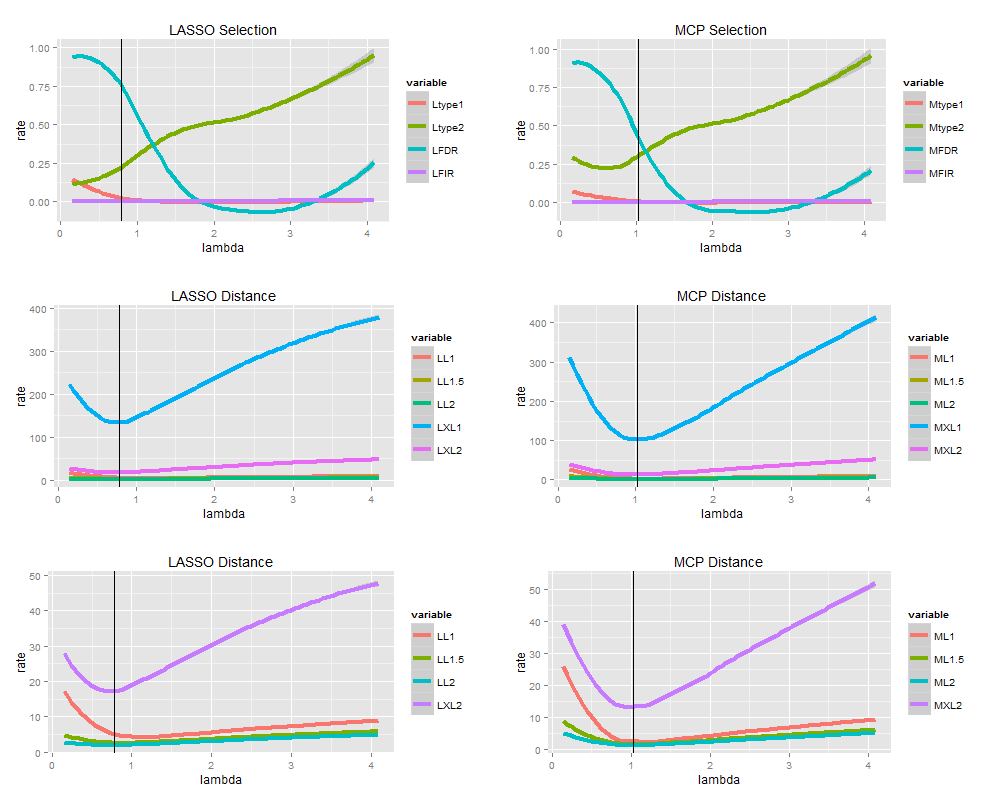
\includegraphics[width = 3.7in]{cov0.png}
\end{center}
\end{frame}

\begin{frame}
\frametitle{Covariance Structure 1}
\begin{center}
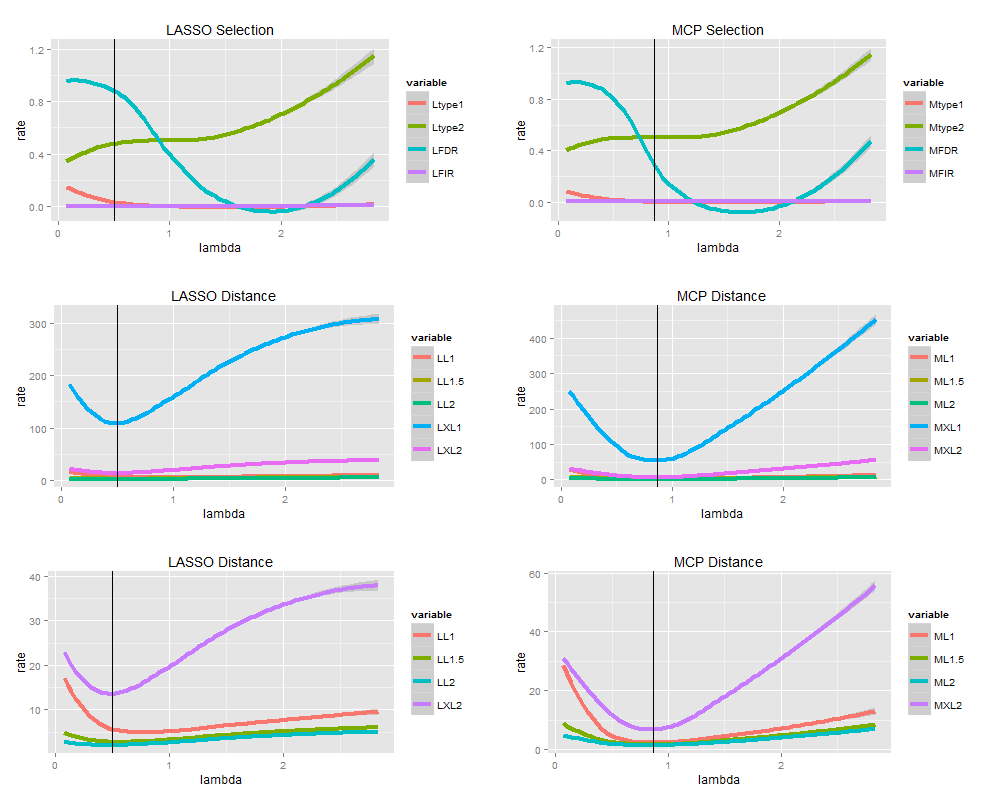
\includegraphics[width = 3.7in]{cov1.png}
\end{center}
\end{frame}

\begin{frame}
\frametitle{Covariance Structure 2}
\begin{center}
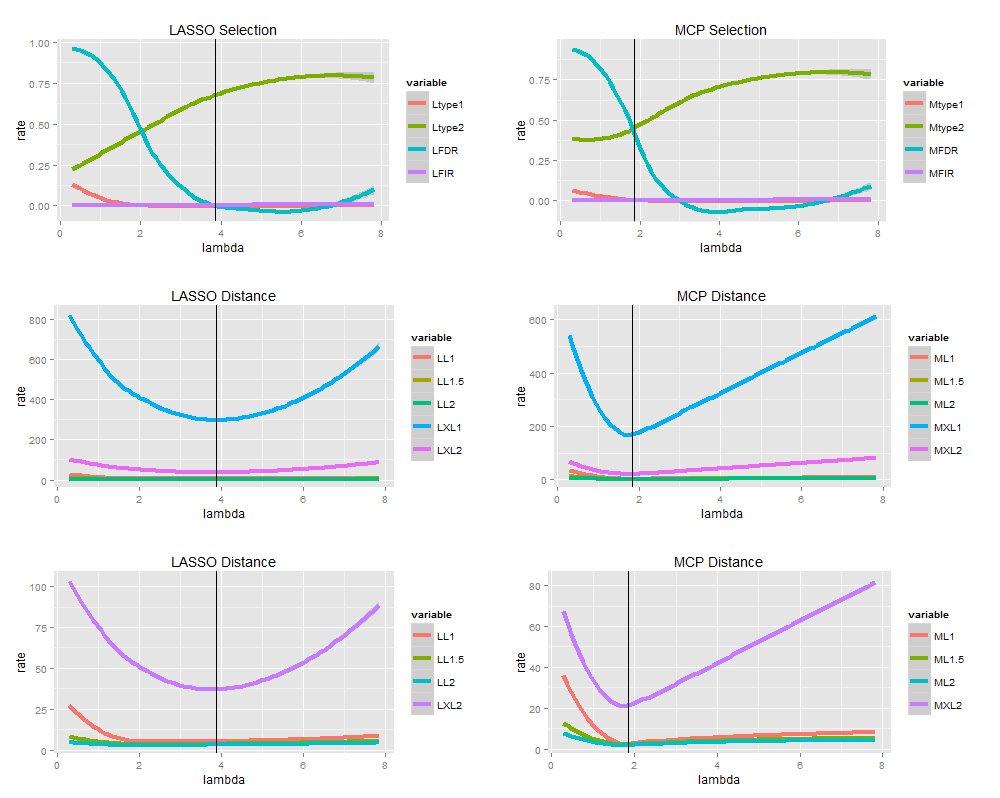
\includegraphics[width = 3.7in]{cov2.png}
\end{center}
\end{frame}

\end{document}
